\documentclass[11pt,a4paper]{article}

% ============ PACKAGES ============
\usepackage[utf8]{inputenc}
\usepackage[T1]{fontenc}
\usepackage[margin=2.2cm]{geometry}
\usepackage{tikz}
\usetikzlibrary{shapes.geometric,arrows.meta,positioning,fit,backgrounds,calc}
\usepackage{hyperref}
\usepackage{xcolor}
\usepackage{enumitem}
\usepackage{booktabs}
\usepackage{array}
\usepackage{titlesec}
\usepackage{fancyhdr}
\usepackage{graphicx}
\usepackage{pdflscape}

\hypersetup{
    colorlinks=true,
    linkcolor=blue!50!black,
    urlcolor=blue!50!black,
    citecolor=blue!50!black
}

\pagestyle{fancy}
\fancyhf{}
\fancyhead[L]{Atelier 1 -- Version 2 : architecture hybride répartie}
\fancyhead[R]{\thepage}
\renewcommand{\headrulewidth}{0.4pt}

\titleformat{\section}{\normalfont\Large\bfseries\color{blue!40!black}}{\thesection}{1em}{}
\titleformat{\subsection}{\normalfont\large\bfseries\color{blue!30!black}}{\thesubsection}{1em}{}

% ============ COULEURS C4 ============
\definecolor{c4person}{RGB}{8,68,102}
\definecolor{c4system}{RGB}{30,111,166}
\definecolor{c4container}{RGB}{68,152,206}
\definecolor{c4external}{RGB}{140,140,140}
\definecolor{c4new}{RGB}{40,140,100}
\definecolor{c4warn}{RGB}{176,88,30}

\tikzstyle{personbox} = [rectangle, rounded corners, minimum width=3.2cm, minimum height=1.6cm,
    text centered, draw=black, fill=c4person, text=white, font=\small, text width=3cm, align=center]
\tikzstyle{systembox} = [rectangle, rounded corners, minimum width=4cm, minimum height=1.8cm,
    text centered, draw=black, fill=c4system, text=white, font=\small, text width=3.8cm, align=center]
\tikzstyle{containerbox} = [rectangle, rounded corners, minimum width=3.4cm, minimum height=1.8cm,
    text centered, draw=black, fill=c4container, text=white, font=\footnotesize, text width=3.2cm, align=center]
\tikzstyle{extbox} = [rectangle, rounded corners, minimum width=3.2cm, minimum height=1.6cm,
    text centered, draw=black, fill=c4external, text=white, font=\small, text width=3cm, align=center]
\tikzstyle{warnbox} = [rectangle, rounded corners, minimum width=3cm, minimum height=1.5cm,
    text centered, draw=black, fill=c4warn, text=white, font=\footnotesize, text width=2.8cm, align=center]
% boîte compacte pour les schémas denses
\tikzstyle{tb} = [rectangle, rounded corners, draw=black, text=white, font=\scriptsize,
    text width=3.0cm, minimum height=1.3cm, align=center, inner sep=3pt]
\tikzstyle{arr} = [-{Latex[length=2.5mm]}, thick, color=black!70]
\tikzstyle{biarr} = [{Latex[length=2.5mm]}-{Latex[length=2.5mm]}, thick, color=black!70]

% ============ INFOS ============
\title{\textbf{Atelier 1 -- Version 2 \\ Migration vers une architecture hybride répartie} \\[0.3cm]
\large Étude de cas : \textit{Parallel Collective Tiny Deep Learning System for Face and Object Reidentification in Uncontrolled Environments}}
\author{Module : Analyse et Modélisation des Architectures Logicielles}
\date{\today}

\begin{document}

\maketitle
\thispagestyle{empty}

\begin{abstract}
\noindent Ce document est la seconde version du travail rendu pour l'Atelier 1. Il porte sur l'article \textit{« Parallel Collective Tiny Deep Learning System for Face and Object Reidentification in Uncontrolled Environments »} (Helaoui \& Bahroun, 2025). La première version proposait de transformer le prototype de l'article en véritables microservices conteneurisés. Cette version 2 va plus loin : elle \textbf{migre la solution vers une architecture hybride, conçue comme un système réparti}, qui combine un style client-serveur (relation dispositif--cloud), des microservices (côté cloud), une communication par événements (publish/subscribe) et une couche Edge/IoT. L'analyse de l'existant est complétée par une lecture selon les propriétés des systèmes répartis (pannes partielles, absence d'horloge globale, cohérence, transparence). La nouvelle architecture est modélisée avec le formalisme C4 et complétée par une vue de déploiement multi-zones, un scénario dynamique et un zoom sur le service de fusion. Des pistes de validation, adaptées aux systèmes répartis, concluent le travail.
\end{abstract}

\tableofcontents
\newpage

% ======================================================================
\section{Introduction}
% ======================================================================

\subsection{Contexte et objectif}

L'article étudié propose un système appelé \textbf{DNN//*Tcs} (\textit{Parallel Collective Tiny Deep Learning client-server System}). Il vise à assister une machine autonome (véhicule autonome, lunettes pour personnes malvoyantes, surveillance intelligente) en combinant en temps réel quatre services de vision :

\begin{itemize}[nosep]
    \item la reconnaissance faciale (\textit{Face Recognition}) ;
    \item la détection d'objets (\textit{Object Detection}) ;
    \item la classification du genre (\textit{Gender Detection}) ;
    \item la reconnaissance d'émotion (\textit{Emotion Recognition}).
\end{itemize}

L'idée centrale est de faire tourner \textbf{plusieurs versions} de chaque service en parallèle -- une version légère (\textit{lite}) sur le dispositif et plusieurs versions plus précises sur un serveur -- puis de \textbf{combiner leurs résultats} (approche « collective »). Des micro-contrôleurs (Arduino) attachés aux objets réels (« Tiny objects ») fournissent en plus une donnée de référence (identité, position, dimensions).

L'atelier demande : (1) d'analyser l'architecture utilisée, (2) de modéliser une nouvelle architecture, (3) de proposer des idées de validation, (4) de livrer le travail en un seul fichier \LaTeX. Pour cette version 2, la nouvelle architecture est \textbf{explicitement conçue comme un système réparti hybride}.

\subsection{Ce qui change par rapport à la version 1}

\begin{table}[h]
\centering
\begin{tabular}{|p{3.0cm}|p{5.6cm}|p{6.0cm}|}
\hline
\textbf{Aspect} & \textbf{Version 1} & \textbf{Version 2 (ce document)} \\
\hline
Style visé & Microservices conteneurisés derrière un Gateway, relation client-serveur conservée & \textbf{Hybride réparti} : Edge--Cloud, microservices, événementiel (pub/sub), IoT \\
\hline
Répartition & Un serveur « logique » dupliqué derrière un Load Balancer & \textbf{Trois tiers} (terrain, edge, cloud) et \textbf{cloud multi-zones} avec réplication \\
\hline
Lecture de l'existant & Critères microservices (5 critères) & Idem, \textbf{plus} lecture selon les 8 propriétés des systèmes répartis \\
\hline
Pannes & Tests de résilience en validation & \textbf{Conçues dans l'architecture} : échéances, reprises idempotentes, circuit breaker, modes dégradés \\
\hline
Cohérence des données & Une base par service & \textbf{Choix explicite} par type de donnée (théorème CAP) \\
\hline
Temps et ordre & Non traités & Identifiant de corrélation et horodatage pour fusionner des résultats venus de machines différentes \\
\hline
Diagrammes & Contexte, conteneurs, composants (existant) ; contexte, conteneurs (nouveau) & + \textbf{vue de déploiement multi-zones}, \textbf{scénario dynamique}, \textbf{composants du service de Fusion} \\
\hline
Validation & 8 pistes & 10 pistes, dont partition réseau, doublons, bascule de zone, + \textbf{indicateurs cibles} \\
\hline
\end{tabular}
\caption{Évolutions entre la version 1 et la version 2}
\end{table}

% ======================================================================
\section{Partie 1 -- Analyse de l'architecture existante}
% ======================================================================

\subsection{Identification du style architectural}

\subsubsection{Le niveau global : une architecture client-serveur à trois tiers}

Au niveau global, l'architecture est une \textbf{architecture client-serveur} -- le « cs » de \textit{DNN//*Tcs} signifie \textit{client-server}. Mais ce n'est pas un client-serveur classique :

\begin{itemize}
    \item \textbf{Le client est un client lourd.} L'application mobile exécute elle-même des modèles légers (\textit{DNN//c}) et produit un résultat local complet, avant d'avoir reçu la réponse du serveur.
    \item \textbf{Le serveur agit comme correcteur.} Il refait le calcul avec des modèles plus précis (\textit{DNN//s}) et ne renvoie une \textit{alerte} que s'il détecte un désaccord.
    \item \textbf{Un troisième tier existe : les objets connectés (Tiny/IoT).} Les micro-contrôleurs Arduino forment une couche « terrain » qui communique avec le client (couche \textit{edge}) et avec le serveur (couche \textit{cloud}).
    \item \textbf{L'accès au serveur passe par une \textit{Gateway} et des \textit{endpoints} REST} (Figures 1 et 2 de l'article).
\end{itemize}

\textbf{Formule retenue :} \textit{« Une architecture client-serveur à client lourd, étendue à trois tiers par l'ajout d'objets connectés (Tiny), avec un accès au serveur structuré par une API Gateway et des services REST. »}

\subsubsection{Le point clé : « microservices » dans le nom, pas dans les faits}

Les auteurs emploient le terme « micro-service » partout (préfixe \texttt{MS} : \texttt{MSLBPHFaceRecognition}, \texttt{MSShowResult}, \texttt{MSParallelCollectiveManager}\ldots). Il faut distinguer deux niveaux :

\begin{table}[h]
\centering
\begin{tabular}{|p{3.4cm}|p{11.2cm}|}
\hline
\textbf{Niveau} & \textbf{Constat} \\
\hline
\textbf{Intention / conception} & Les auteurs \emph{pensent} leur système comme des microservices : quatre services métier (visage, objet, genre, émotion), une \textit{Gateway}, des \textit{endpoints} REST. \\
\hline
\textbf{Implémentation réelle} (section 6 de l'article) & Le prototype tourne sur \textbf{une seule machine} (portable Dell Vostro 3400, Intel i3 à 4 cœurs), en \textbf{Python} avec \texttt{multiprocessing}. Les « micro-services » sont des \textbf{fonctions qui s'appellent directement} (\texttt{RunProcess2(...)}, \texttt{RunProcess3(...)}), sans réseau. \\
\hline
\end{tabular}
\caption{Intention et réalité de l'implémentation}
\end{table}

En confrontant l'implémentation aux cinq critères reconnus d'une architecture microservices (Fowler \& Lewis) :

\begin{table}[h]
\centering
\begin{tabular}{|p{4.8cm}|p{6.4cm}|p{1.4cm}|}
\hline
\textbf{Critère} & \textbf{Ce que fait le prototype (section 6)} & \textbf{Respecté} \\
\hline
Déployable indépendamment & Tout fait partie du même programme, lancé et arrêté ensemble & \textbf{Non} \\
\hline
Communique par le réseau & Appels de fonctions directs en mémoire & \textbf{Non} \\
\hline
Propriétaire de ses données & Le dossier du \textit{dataset} de visages est \textbf{partagé} entre plusieurs « MS » (Algorithmes 3 et 5) & \textbf{Non} \\
\hline
Scalable indépendamment & Règle rigide « un service = un processeur » & \textbf{Non} \\
\hline
Isolé en cas de panne & \texttt{MSDetectGender} appelle \texttt{MSDNNDetectFaces} qui rappelle \texttt{MSDetectGender} : si un maillon casse, la boucle s'arrête (Algorithmes 9-10) & \textbf{Non} \\
\hline
\end{tabular}
\caption{Confrontation de l'implémentation aux 5 critères d'un microservice}
\end{table}

\textbf{Aucun critère n'est rempli.} Exemple révélateur : après le ré-entraînement dynamique (\texttt{MSFaceDynamicTraining}), les auteurs écrivent « \textit{we restart all the service with updated data} » : \textbf{tout le service redémarre}.

\textbf{Conclusion à retenir :} le terme exact pour l'implémentation est un « \textbf{monolithe modulaire multi-processus} ». Seul le \emph{découpage fonctionnel} en quatre services métier derrière une Gateway REST relève de l'esprit microservices. Ce n'est pas non plus du SOA (pas d'\textit{Enterprise Service Bus}).

\subsection{Diagramme C4 -- Niveau 1 : Contexte}

Le niveau Contexte montre le système comme une « boîte noire » et ses interactions avec l'extérieur. Il ne dépend pas des détails internes.

\begin{figure}[h]
\centering
\resizebox{\textwidth}{!}{%
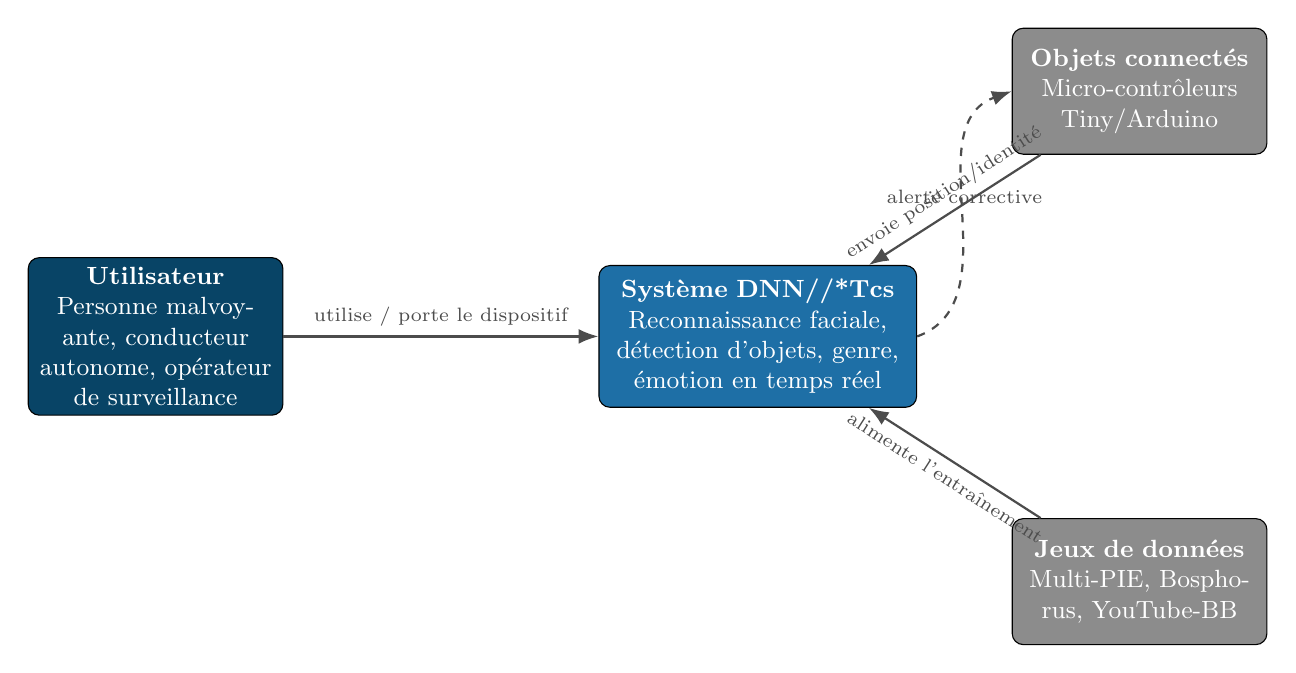
\begin{tikzpicture}[node distance=2.2cm and 2.8cm]

\node[personbox] (user) {\textbf{Utilisateur}\\ Personne malvoyante, conducteur autonome, opérateur de surveillance};

\node[systembox, right=of user, xshift=1.2cm] (system) {\textbf{Système DNN//*Tcs}\\ Reconnaissance faciale, détection d'objets, genre, émotion en temps réel};

\node[extbox, above right=1.4cm and 1.2cm of system] (tiny) {\textbf{Objets connectés}\\ Micro-contrôleurs Tiny/Arduino};

\node[extbox, below right=1.4cm and 1.2cm of system] (dataset) {\textbf{Jeux de données}\\ Multi-PIE, Bosphorus, YouTube-BB};

\draw[arr] (user) -- node[above, font=\scriptsize] {utilise / porte le dispositif} (system);
\draw[arr] (tiny) -- node[above, sloped, font=\scriptsize] {envoie position/identité} (system);
\draw[arr] (dataset) -- node[below, sloped, font=\scriptsize] {alimente l'entraînement} (system);
\draw[arr, dashed] (system.east) to[out=20,in=200] node[above, font=\scriptsize] {alerte corrective} (tiny.west);

\end{tikzpicture}
}
\caption{Diagramme C4 -- Niveau Contexte de l'architecture existante}
\end{figure}

\subsection{Diagramme C4 -- Niveau 2 : Conteneurs}

Un « conteneur » C4 est une unité \textbf{déployable indépendamment}. Le serveur de l'article n'étant qu'\textbf{une seule unité de déploiement}, il est représenté par \textbf{un unique conteneur}.

\begin{figure}[h]
\centering
\resizebox{0.92\textwidth}{!}{%
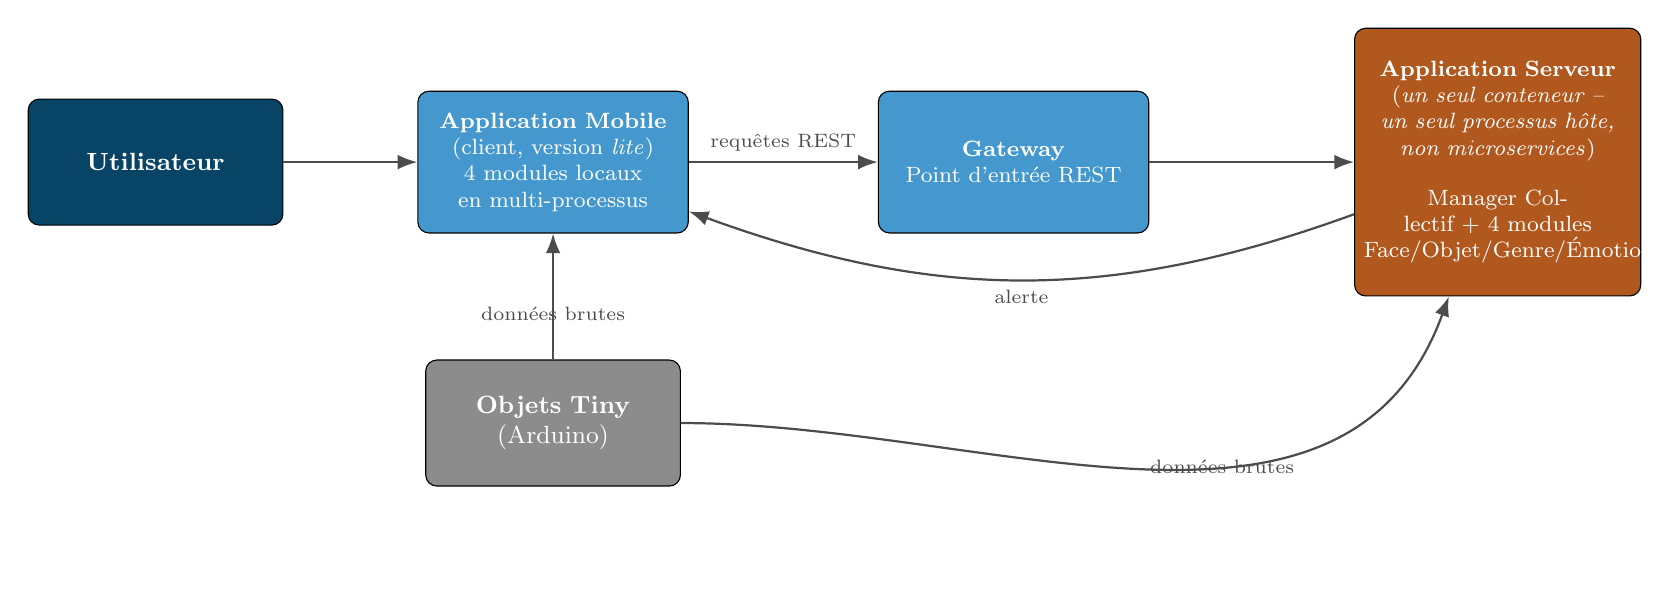
\begin{tikzpicture}[node distance=1.3cm and 1.4cm]

\node[personbox] (user) {\textbf{Utilisateur}};

\node[containerbox, right=of user, xshift=0.3cm] (mobile) {\textbf{Application Mobile}\\ (client, version \textit{lite})\\ 4 modules locaux en multi-processus};

\node[containerbox, right=2.4cm of mobile] (gateway) {\textbf{Gateway}\\ Point d'entrée REST};

\node[warnbox, right=2.6cm of gateway, minimum height=3.4cm, text width=3.4cm] (server) {\textbf{Application Serveur}\\ \footnotesize (\emph{un seul conteneur -- un seul processus hôte, non microservices})\\[0.3cm] Manager Collectif + 4 modules Face/Objet/Genre/Émotion};

\node[extbox, below=1.6cm of mobile] (tiny) {\textbf{Objets Tiny}\\ (Arduino)};

\draw[arr] (user) -- (mobile);
\draw[arr] (mobile) -- node[above, font=\scriptsize] {requêtes REST} (gateway);
\draw[arr] (gateway) -- (server);
\draw[arr] (server) to[out=200,in=340] node[below, font=\scriptsize] {alerte} (mobile);
\draw[arr] (tiny) -- node[below, font=\scriptsize] {données brutes} (mobile);
\draw[arr] (tiny) to[out=0,in=250] node[right, font=\scriptsize] {données brutes} (server);

\end{tikzpicture}
}
\caption{Diagramme C4 -- Niveau Conteneurs de l'architecture existante (le serveur est un seul conteneur)}
\end{figure}

\subsection{Diagramme C4 -- Niveau 3 : Composants (intérieur du conteneur serveur)}

\textit{Complément non exigé par l'énoncé :} ce zoom rend visible le « monolithe modulaire ».

\begin{figure}[h]
\centering
\resizebox{0.95\textwidth}{!}{%
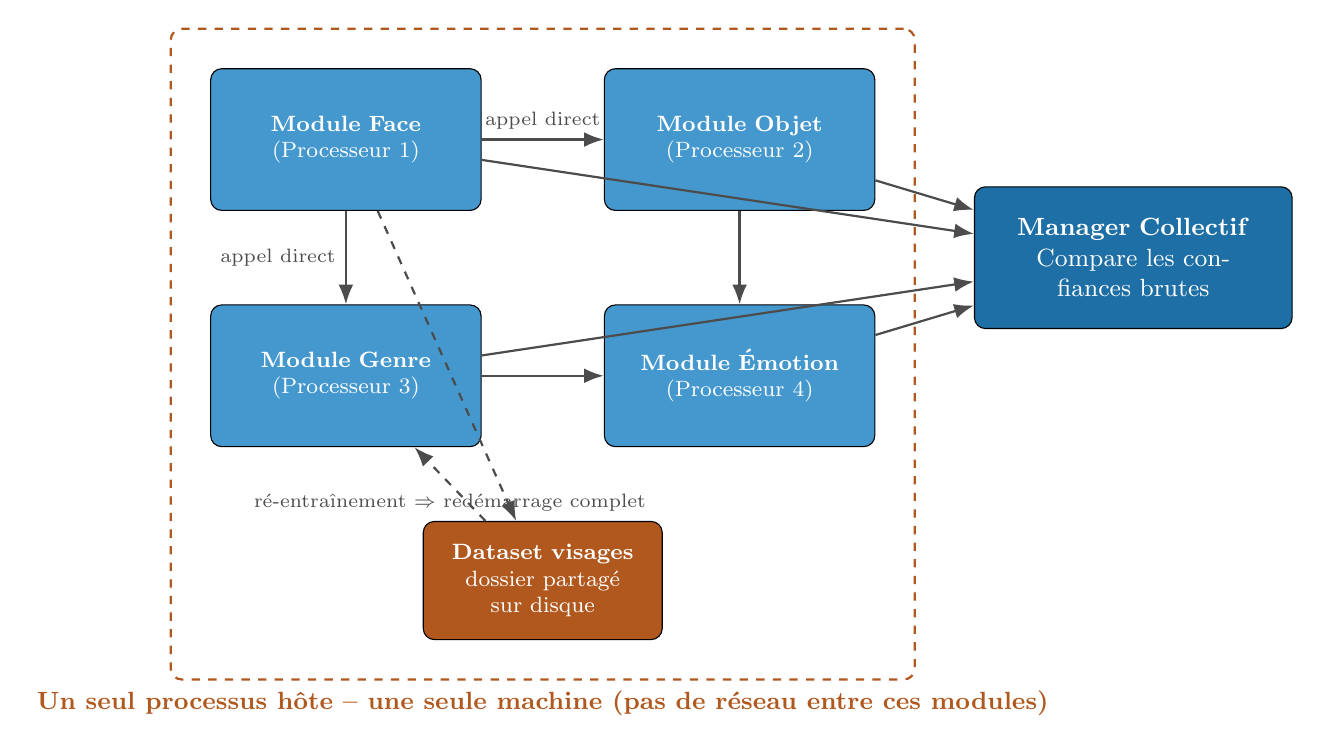
\begin{tikzpicture}[node distance=1.1cm and 1.1cm]

\node[containerbox] (face) at (0,3) {\textbf{Module Face}\\ (Processeur 1)};
\node[containerbox] (obj) at (5,3) {\textbf{Module Objet}\\ (Processeur 2)};
\node[containerbox] (gender) at (0,0) {\textbf{Module Genre}\\ (Processeur 3)};
\node[containerbox] (emotion) at (5,0) {\textbf{Module Émotion}\\ (Processeur 4)};

\node[systembox, fill=c4system] (manager) at (10,1.5) {\textbf{Manager Collectif}\\ Compare les confiances brutes};

\node[warnbox] (dataset) at (2.5,-2.6) {\textbf{Dataset visages}\\ dossier partagé sur disque};

\draw[arr] (face) -- node[above, font=\scriptsize] {appel direct} (obj);
\draw[arr] (face) -- node[left, font=\scriptsize] {appel direct} (gender);
\draw[arr] (obj) -- (emotion);
\draw[arr] (gender) -- (emotion);
\draw[arr] (face) -- (manager);
\draw[arr] (obj) -- (manager);
\draw[arr] (gender) -- (manager);
\draw[arr] (emotion) -- (manager);
\draw[arr, dashed] (face) -- (dataset);
\draw[arr, dashed] (dataset) -- node[below, font=\scriptsize] {ré-entraînement $\Rightarrow$ redémarrage complet} (gender);

\begin{scope}[on background layer]
\node[draw=c4warn, thick, dashed, rounded corners, fit=(face)(obj)(gender)(emotion)(dataset), inner sep=0.5cm, label={[c4warn, font=\bfseries\small]below:Un seul processus hôte -- une seule machine (pas de réseau entre ces modules)}] {};
\end{scope}

\end{tikzpicture}
}
\caption{Diagramme C4 -- Niveau Composants : l'intérieur du « monolithe modulaire » serveur}
\end{figure}

\subsection{Description des composants principaux}

\begin{itemize}
    \item \textbf{Application mobile (client lourd)} : exécute une version allégée de chaque module (un processus par cœur), calcule un résultat local et l'envoie au serveur.
    \item \textbf{Gateway} : point d'entrée unique vers l'application serveur.
    \item \textbf{Application serveur (monolithe modulaire multi-processus)} : quatre modules (Face, Objet, Genre, Émotion), chacun pouvant exécuter plusieurs versions d'un algorithme (LBPH + CNN, YOLOv8n/m/l/x\ldots), tous dans le même processus hôte.
    \item \textbf{Manager Collectif} (\texttt{MSParallelCollectiveManager}) : sélectionne le résultat de meilleure confiance \emph{brute} et notifie le client en cas d'erreur.
    \item \textbf{Objets Tiny (Arduino)} : envoient identité, position, dimensions -- une « vérité terrain » légère.
\end{itemize}

\subsection{Lecture sous l'angle des systèmes répartis}

Un système réparti est un ensemble de machines indépendantes qui coopèrent par échange de messages et se présentent à l'utilisateur comme un système unique. Ses difficultés viennent de trois faits : les machines tombent en panne \emph{séparément}, il n'existe \emph{pas d'horloge commune}, et le réseau est \emph{lent et peu fiable}. Le tableau confronte l'article à huit propriétés classiques.

\begin{table}[h]
\centering
\begin{tabular}{|p{2.7cm}|p{3.7cm}|p{6.3cm}|p{1.4cm}|}
\hline
\textbf{Propriété} & \textbf{Question posée} & \textbf{Dans l'article} & \textbf{Verdict} \\
\hline
Hétérogénéité & Matériels, systèmes et réseaux différents cohabitent-ils ? & Arduino, smartphone, serveur : oui, mais aucun protocole commun n'est spécifié pour le canal Tiny & Partiel \\
\hline
Concurrence & Plusieurs activités s'exécutent-elles en même temps ? & Très forte (multi-processus, N versions), mais sur \emph{une seule machine} et sans coordination répartie & Partiel \\
\hline
Horloge globale & Comment ordonner des résultats venus de machines différentes ? & Non traité : aucun identifiant de corrélation ni horodatage pour fusionner client, serveur et Tiny & Non \\
\hline
Pannes partielles & Que se passe-t-il si un nœud tombe ? & Non traité : Manager unique, pas de réplication, pas de délai maximal d'attente & Non \\
\hline
Transparence & L'utilisateur ignore-t-il où tourne chaque chose (localisation, réplication, panne) ? & Non : adresses fixes, pas de registre de services & Non \\
\hline
Passage à l'échelle & Le système tient-il avec beaucoup de clients ? & Formules $P^*_c$ et $P^*_s$ calculées pour \emph{un seul} client & Partiel \\
\hline
Sécurité & Échanges et identités sont-ils protégés ? & Non traité (visages = données biométriques) & Non \\
\hline
Ouverture & Peut-on ajouter une version sans toucher au reste ? & Non : ajouter un modèle revient à modifier le programme & Faible \\
\hline
\end{tabular}
\caption{L'article analysé selon les propriétés des systèmes répartis}
\end{table}

\textbf{Constat :} le système est \emph{distribué géographiquement} (client, serveur, objets) mais il n'est \emph{pas conçu comme un système réparti}. La répartition est subie, non maîtrisée. C'est précisément ce que la version 2 corrige.

\subsection{Limites identifiées}

L'article valide l'efficacité \emph{algorithmique} de la solution mais traite peu les aspects \emph{architecturaux}. Chaque limite est associée à une piste de correction qui prépare la partie 2.

\begin{table}[h]
\centering
\begin{tabular}{|p{4.6cm}|p{4.6cm}|p{4.6cm}|}
\hline
\textbf{Limite identifiée} & \textbf{Pourquoi c'est un problème} & \textbf{Piste de correction} \\
\hline
Pas réellement microservices : monolithe modulaire multi-processus sur une machine &
Aucun déploiement indépendant, aucune communication réseau, aucune isolation des pannes &
\textbf{Conteneuriser} chaque service, communication par le réseau \\
\hline
Point d'entrée unique (\textit{Gateway}) sans équilibrage de charge &
Si le Gateway tombe, tout le système est inaccessible (\textit{Single Point of Failure}) &
\textbf{Load Balancer} et plusieurs instances, réparties sur plusieurs zones \\
\hline
Communication synchrone (REST) entre Manager et modules &
Le Manager attend toutes les réponses : latence cumulée, couplage fort &
\textbf{Bus d'événements} (publish/subscribe), échanges asynchrones \\
\hline
Dataset de visages partagé, sans propriétaire, sans réplication, sans modèle de cohérence &
Conflits d'accès, perte de données, états divergents &
\textbf{Une base par service}, réplication, \textbf{cohérence choisie} par type de donnée \\
\hline
Redémarrage complet du service au ré-entraînement (« \textit{restart all the service} ») &
Tous les modules s'interrompent pour mettre à jour un seul modèle &
\textbf{Mise à jour à chaud} et déploiement progressif d'un modèle \\
\hline
Fusion naïve : « meilleure confiance » brute entre modèles hétérogènes (LBPH, CNN, YOLO) &
Les scores de modèles différents ne sont pas calibrés sur la même échelle &
\textbf{Calibrer} les scores puis faire un \textbf{vote pondéré} \\
\hline
Pannes partielles non traitées : pas d'échéance, pas de reprise, Manager serveur unique &
Un service lent ou tombé bloque la décision collective &
\textbf{Échéance} de collecte, \textit{circuit breaker}, \textbf{modes dégradés}, Manager répliqué \\
\hline
Pas d'identifiant de corrélation, d'horodatage, ni gestion des doublons &
Impossible de savoir à quelle image correspond un résultat tardif ou dupliqué &
\texttt{frame\_id} unique, horodatage, consommateurs \textbf{idempotents} \\
\hline
Aucune sécurité (chiffrement, authentification des objets Tiny, biométrie) &
Un objet falsifié peut tromper le Manager ; fuite de données de visages &
\textbf{mTLS}, identité des appareils, envoi d'\textbf{embeddings} plutôt que d'images \\
\hline
Aucune supervision &
Impossible de savoir quel nœud est lent ou dégrade la précision &
\textbf{Observabilité} : logs, métriques, traces distribuées \\
\hline
Scalabilité multi-clients non étudiée, règle « un module = un processeur » &
Le nombre de processeurs explose avec les clients &
\textbf{Scaling horizontal} indépendant de chaque service, partitionnement par client \\
\hline
\end{tabular}
\caption{Limites de l'architecture existante et pistes de correction}
\end{table}

% ======================================================================
\section{Partie 2 -- Nouvelle architecture hybride répartie}
% ======================================================================

\subsection{Pourquoi une architecture hybride répartie ?}

Une architecture « hybride » combine plusieurs styles là où chacun est le plus pertinent. Le système a des besoins contradictoires : réagir \emph{tout de suite} (un malvoyant ne peut pas attendre le réseau) et \emph{être très précis} (ce qui exige de la puissance de calcul distante). Aucun style unique ne couvre les deux. On les combine donc :

\begin{table}[h]
\centering
\begin{tabular}{|p{3.6cm}|p{4.6cm}|p{6.4cm}|}
\hline
\textbf{Style} & \textbf{Où on l'utilise} & \textbf{Ce qu'il apporte} \\
\hline
Client-serveur & Entre le dispositif et le cloud & Séparation claire entre client lourd (décision locale) et serveur (correction) -- on conserve ce qui fonctionne \\
\hline
Edge / IoT & Objets Tiny et dispositif de l'utilisateur & Traitement au plus près de la source : faible latence, fonctionnement hors ligne \\
\hline
Microservices & Côté cloud (inférence, fusion, alertes) & Déploiement, évolution et mise à l'échelle indépendants de chaque service \\
\hline
Événementiel (publish/subscribe) & Colonne vertébrale entre tous les services & Découplage : une même image est traitée par N versions sans que les services se connaissent \\
\hline
Système réparti (réplication, quorum) & Cloud sur plusieurs zones & Tolérance aux pannes, disponibilité, passage à l'échelle \\
\hline
\end{tabular}
\caption{Les styles combinés et leur rôle}
\end{table}

La comparaison avec les alternatives justifie ce choix :

\begin{table}[h]
\centering
\begin{tabular}{|p{3.4cm}|p{1.9cm}|p{2.2cm}|p{2.3cm}|p{1.9cm}|p{2.0cm}|}
\hline
\textbf{Architecture} & \textbf{Temps réel} & \textbf{Extensibilité} & \textbf{Tolérance aux pannes} & \textbf{Échelle} & \textbf{Verdict} \\
\hline
Monolithe sur le dispositif & Bon & Très faible & Faible & Non & Rejetée \\
\hline
Client-serveur REST (existant) & Moyen & Faible & Faible & Limitée & À améliorer \\
\hline
Microservices 100\% cloud & Mauvais (dépend du réseau) & Très bonne & Bonne & Très bonne & Rejetée \\
\hline
\textbf{Hybride réparti} & \textbf{Bon} (décision locale) & \textbf{Très bonne} & \textbf{Bonne} (réplication) & \textbf{Très bonne} & \textbf{Retenue} \\
\hline
\end{tabular}
\caption{Comparaison des architectures candidates}
\end{table}

\subsection{Principes directeurs}

\begin{enumerate}
    \item \textbf{Décision locale d'abord, cloud pour corriger.} Le dispositif ne dépend jamais du cloud pour agir.
    \item \textbf{Tout ce qui est partagé passe par des événements.} Les services ne s'appellent pas directement : ils publient et s'abonnent.
    \item \textbf{Chaque service possède ses données, est sans état et réplicable.}
    \item \textbf{La panne partielle est la règle, pas l'exception.} Échéances, reprises idempotentes, \textit{circuit breaker} et modes dégradés sont prévus dès la conception.
    \item \textbf{La cohérence est choisie selon la donnée} (théorème CAP, voir 3.8).
    \item \textbf{Sécurité et vie privée dès la conception} : chiffrement, identité des appareils, minimisation des données biométriques.
    \item \textbf{Observer pour prouver} : chaque message porte un identifiant de corrélation, et les traces sont reconstituables de bout en bout.
\end{enumerate}

\subsection{Vue d'ensemble : trois tiers et diagramme C4 de contexte}

Le système est réparti sur trois tiers selon la distance au terrain : plus on s'éloigne de l'utilisateur, plus on gagne en puissance, mais plus la latence augmente.

\begin{table}[h]
\centering
\begin{tabular}{|p{2.6cm}|p{4.3cm}|p{3.9cm}|p{3.5cm}|}
\hline
\textbf{Tier} & \textbf{Contenu} & \textbf{Atout} & \textbf{Contrainte} \\
\hline
1 -- Terrain (IoT) & Objets Tiny (Arduino) & Donnée de référence très légère & Ressources minimales \\
\hline
2 -- Edge & Dispositif de l'utilisateur (mobile, lunettes) & Latence minimale, autonomie & Calcul et batterie limités \\
\hline
3 -- Cloud & Services répliqués sur plusieurs zones & Puissance, précision, élasticité & Latence, dépendance au réseau \\
\hline
\end{tabular}
\caption{Les trois tiers de la nouvelle architecture}
\end{table}

Le contexte (niveau 1) reste proche de la version 1 : la mission et les acteurs ne changent pas, seul l'intérieur est transformé. Un acteur apparaît : l'\textbf{administrateur système}, rendu nécessaire par la supervision d'un système réparti.

\begin{figure}[h]
\centering
\resizebox{\textwidth}{!}{%
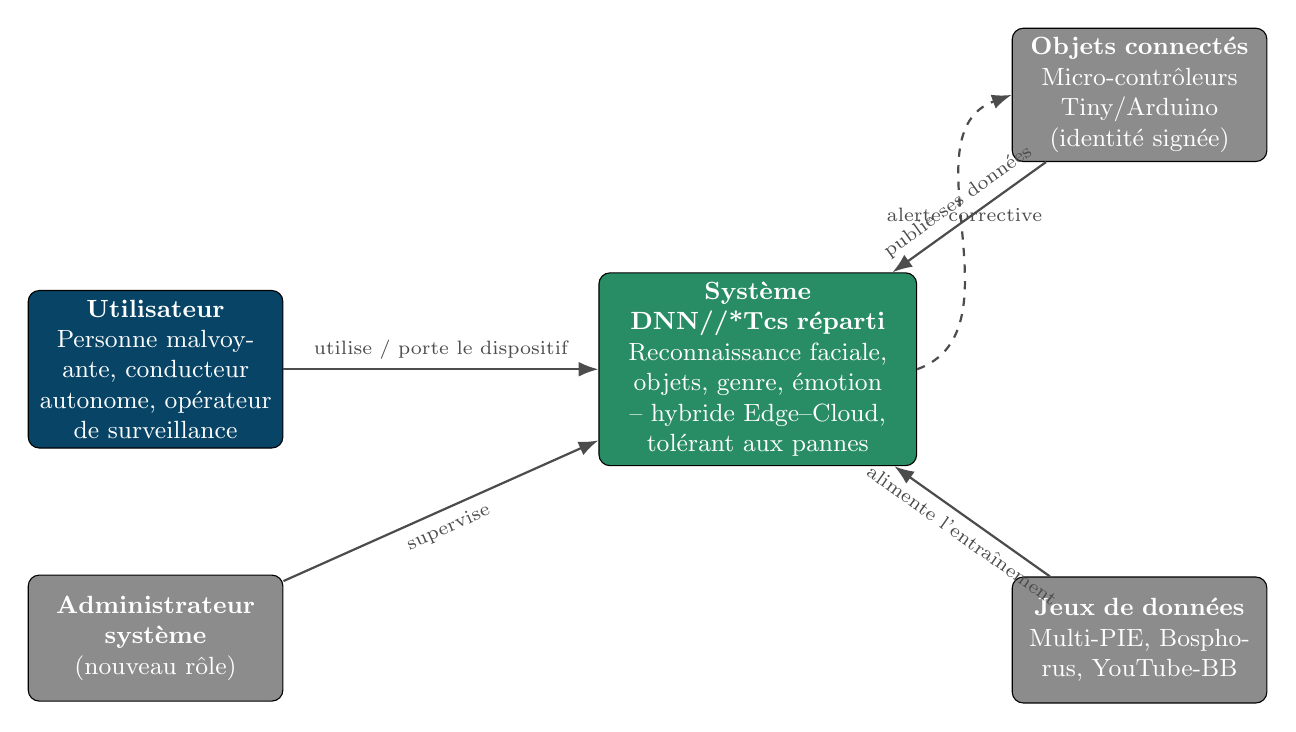
\begin{tikzpicture}[node distance=2.2cm and 2.8cm]

\node[personbox] (user) {\textbf{Utilisateur}\\ Personne malvoyante, conducteur autonome, opérateur de surveillance};

\node[systembox, right=of user, xshift=1.2cm, fill=c4new] (system) {\textbf{Système DNN//*Tcs réparti}\\ Reconnaissance faciale, objets, genre, émotion -- hybride Edge--Cloud, tolérant aux pannes};

\node[extbox, above right=1.4cm and 1.2cm of system] (tiny) {\textbf{Objets connectés}\\ Micro-contrôleurs Tiny/Arduino (identité signée)};

\node[extbox, below right=1.4cm and 1.2cm of system] (dataset) {\textbf{Jeux de données}\\ Multi-PIE, Bosphorus, YouTube-BB};

\node[extbox, below=1.6cm of user] (admin) {\textbf{Administrateur système}\\ (nouveau rôle)};

\draw[arr] (user) -- node[above, font=\scriptsize] {utilise / porte le dispositif} (system);
\draw[arr] (tiny) -- node[above, sloped, font=\scriptsize] {publie ses données} (system);
\draw[arr] (dataset) -- node[below, sloped, font=\scriptsize] {alimente l'entraînement} (system);
\draw[arr, dashed] (system.east) to[out=20,in=200] node[above, font=\scriptsize] {alerte corrective} (tiny.west);
\draw[arr] (admin) -- node[below, sloped, font=\scriptsize] {supervise} (system);

\end{tikzpicture}
}
\caption{Diagramme C4 -- Niveau Contexte de la nouvelle architecture}
\end{figure}

\subsection{Diagramme C4 -- Niveau 2 : Conteneurs (nouvelle architecture)}

Le schéma ci-après (page suivante, en paysage) montre les trois tiers. Chaque rectangle est une unité déployable indépendamment. Code couleur : gris = terrain, bleu clair = edge, vert = services cloud, bleu foncé = services transverses (registre, MLOps, observabilité). Les services cloud existent en plusieurs réplicas répartis sur plusieurs zones (voir 3.5).

\begin{landscape}
\begin{figure}[p]
\centering
\resizebox{\linewidth}{!}{%
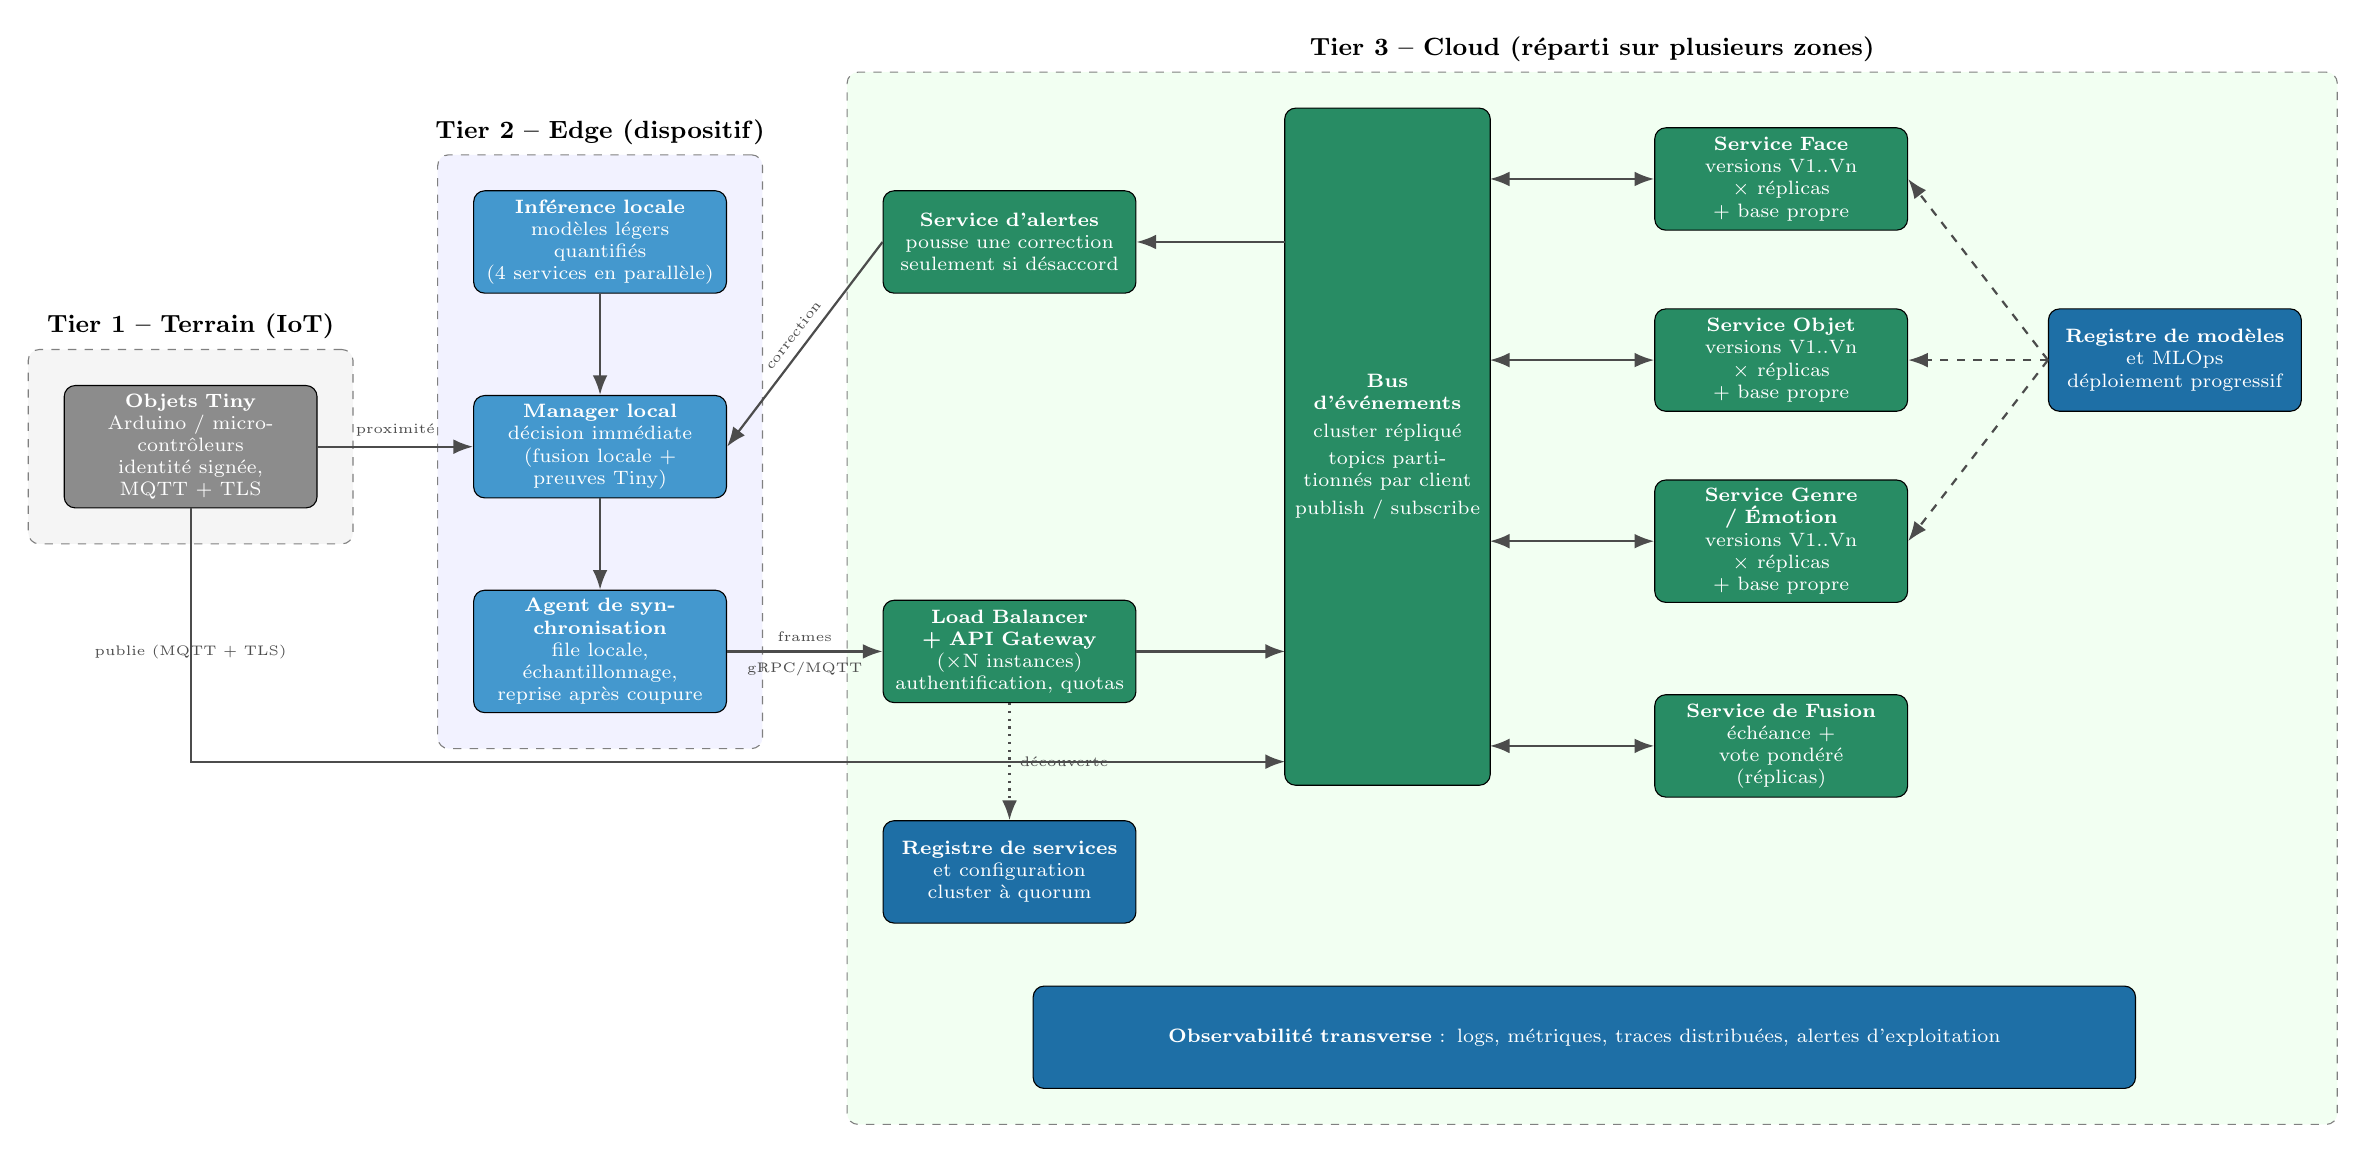
\begin{tikzpicture}[every node/.style={align=center}]

% ---- Tier 1 : terrain ----
\node[tb, fill=c4external] (tiny) at (0,0) {\textbf{Objets Tiny}\\ Arduino / micro-contrôleurs\\ identité signée, MQTT + TLS};

% ---- Tier 2 : edge ----
\node[tb, fill=c4container] (inf) at (5.2,2.6) {\textbf{Inférence locale}\\ modèles légers quantifiés\\ (4 services en parallèle)};
\node[tb, fill=c4container] (mgr) at (5.2,0) {\textbf{Manager local}\\ décision immédiate\\ (fusion locale + preuves Tiny)};
\node[tb, fill=c4container] (sync) at (5.2,-2.6) {\textbf{Agent de synchronisation}\\ file locale, échantillonnage,\\ reprise après coupure};

% ---- Tier 3 : cloud ----
\node[tb, fill=c4new] (alert) at (10.4,2.6) {\textbf{Service d'alertes}\\ pousse une correction\\ seulement si désaccord};
\node[tb, fill=c4new] (gw) at (10.4,-2.6) {\textbf{Load Balancer + API Gateway}\\ ($\times$N instances)\\ authentification, quotas};
\node[tb, fill=c4system] (reg) at (10.4,-5.4) {\textbf{Registre de services}\\ et configuration\\ cluster à quorum};
\node[tb, fill=c4new, minimum height=8.6cm, minimum width=2.6cm, text width=2.4cm] (bus) at (15.2,0) {\textbf{Bus d'événements}\\[2pt] cluster répliqué\\[2pt] topics partitionnés par client\\[2pt] publish / subscribe};
\node[tb, fill=c4new] (face) at (20.2,3.4) {\textbf{Service Face}\\ versions V1..Vn $\times$ réplicas\\ + base propre};
\node[tb, fill=c4new] (obj) at (20.2,1.1) {\textbf{Service Objet}\\ versions V1..Vn $\times$ réplicas\\ + base propre};
\node[tb, fill=c4new] (gen) at (20.2,-1.2) {\textbf{Service Genre / Émotion}\\ versions V1..Vn $\times$ réplicas\\ + base propre};
\node[tb, fill=c4new] (fus) at (20.2,-3.8) {\textbf{Service de Fusion}\\ échéance + vote pondéré\\ (réplicas)};
\node[tb, fill=c4system] (mlops) at (25.2,1.1) {\textbf{Registre de modèles}\\ et MLOps\\ déploiement progressif};
\node[tb, fill=c4system, minimum width=14cm, text width=13.5cm] (obs) at (17.7,-7.5) {\textbf{Observabilité transverse} : logs, métriques, traces distribuées, alertes d'exploitation};

% ---- liens ----
\draw[arr] (tiny.east) -- node[above, font=\tiny] {proximité} (mgr.west);
\draw[arr] (inf) -- (mgr);
\draw[arr] (mgr) -- (sync);
\draw[arr] (sync.east) -- node[above, font=\tiny] {frames} node[below, font=\tiny] {gRPC/MQTT} (gw.west);
\draw[arr] (gw.east) -- (13.9,-2.6);
\draw[arr, dotted] (gw.south) -- node[right, font=\tiny] {découverte} (reg.north);
\draw[arr] (13.9,2.6) -- (alert.east);
\draw[arr] (alert.west) -- node[above, sloped, font=\tiny] {correction} (mgr.east);
\draw[biarr] (16.5,3.4) -- (face.west);
\draw[biarr] (16.5,1.1) -- (obj.west);
\draw[biarr] (16.5,-1.2) -- (gen.west);
\draw[biarr] (16.5,-3.8) -- (fus.west);
\draw[arr, dashed] (mlops.west) -- (face.east);
\draw[arr, dashed] (mlops.west) -- (obj.east);
\draw[arr, dashed] (mlops.west) -- (gen.east);
\draw[arr] (tiny.south) |- node[below, pos=0.25, font=\tiny] {publie (MQTT + TLS)} (13.9,-4.0);

% ---- fonds des tiers ----
\begin{scope}[on background layer]
\node[draw=black!50, dashed, rounded corners, fill=gray!8, fit=(tiny), inner sep=0.45cm, label={[font=\bfseries\small]above:Tier 1 -- Terrain (IoT)}] {};
\node[draw=black!50, dashed, rounded corners, fill=blue!5, fit=(inf)(mgr)(sync), inner sep=0.45cm, label={[font=\bfseries\small]above:Tier 2 -- Edge (dispositif)}] {};
\node[draw=black!50, dashed, rounded corners, fill=green!5, fit=(alert)(gw)(reg)(bus)(face)(obj)(gen)(fus)(mlops)(obs), inner sep=0.45cm, label={[font=\bfseries\small]above:Tier 3 -- Cloud (réparti sur plusieurs zones)}] {};
\end{scope}

\end{tikzpicture}
}
\caption{Diagramme C4 -- Niveau Conteneurs de la nouvelle architecture hybride répartie (flèches pleines : flux de données ; pointillés fins : découverte ; tirets : déploiement des modèles)}
\end{figure}
\end{landscape}

\subsection{Vue de déploiement : répartition sur trois zones}

Les diagrammes C4 montrent la \emph{structure logique}. Pour un système réparti, il faut aussi montrer le \emph{placement physique}. Le cloud est réparti sur \textbf{trois zones de disponibilité} (centres de données indépendants). Trois est le nombre minimal pour un \textbf{quorum} : tant que deux zones sur trois fonctionnent, le registre de services et le bus peuvent prendre des décisions.

\begin{figure}[h]
\centering
\resizebox{\textwidth}{!}{%
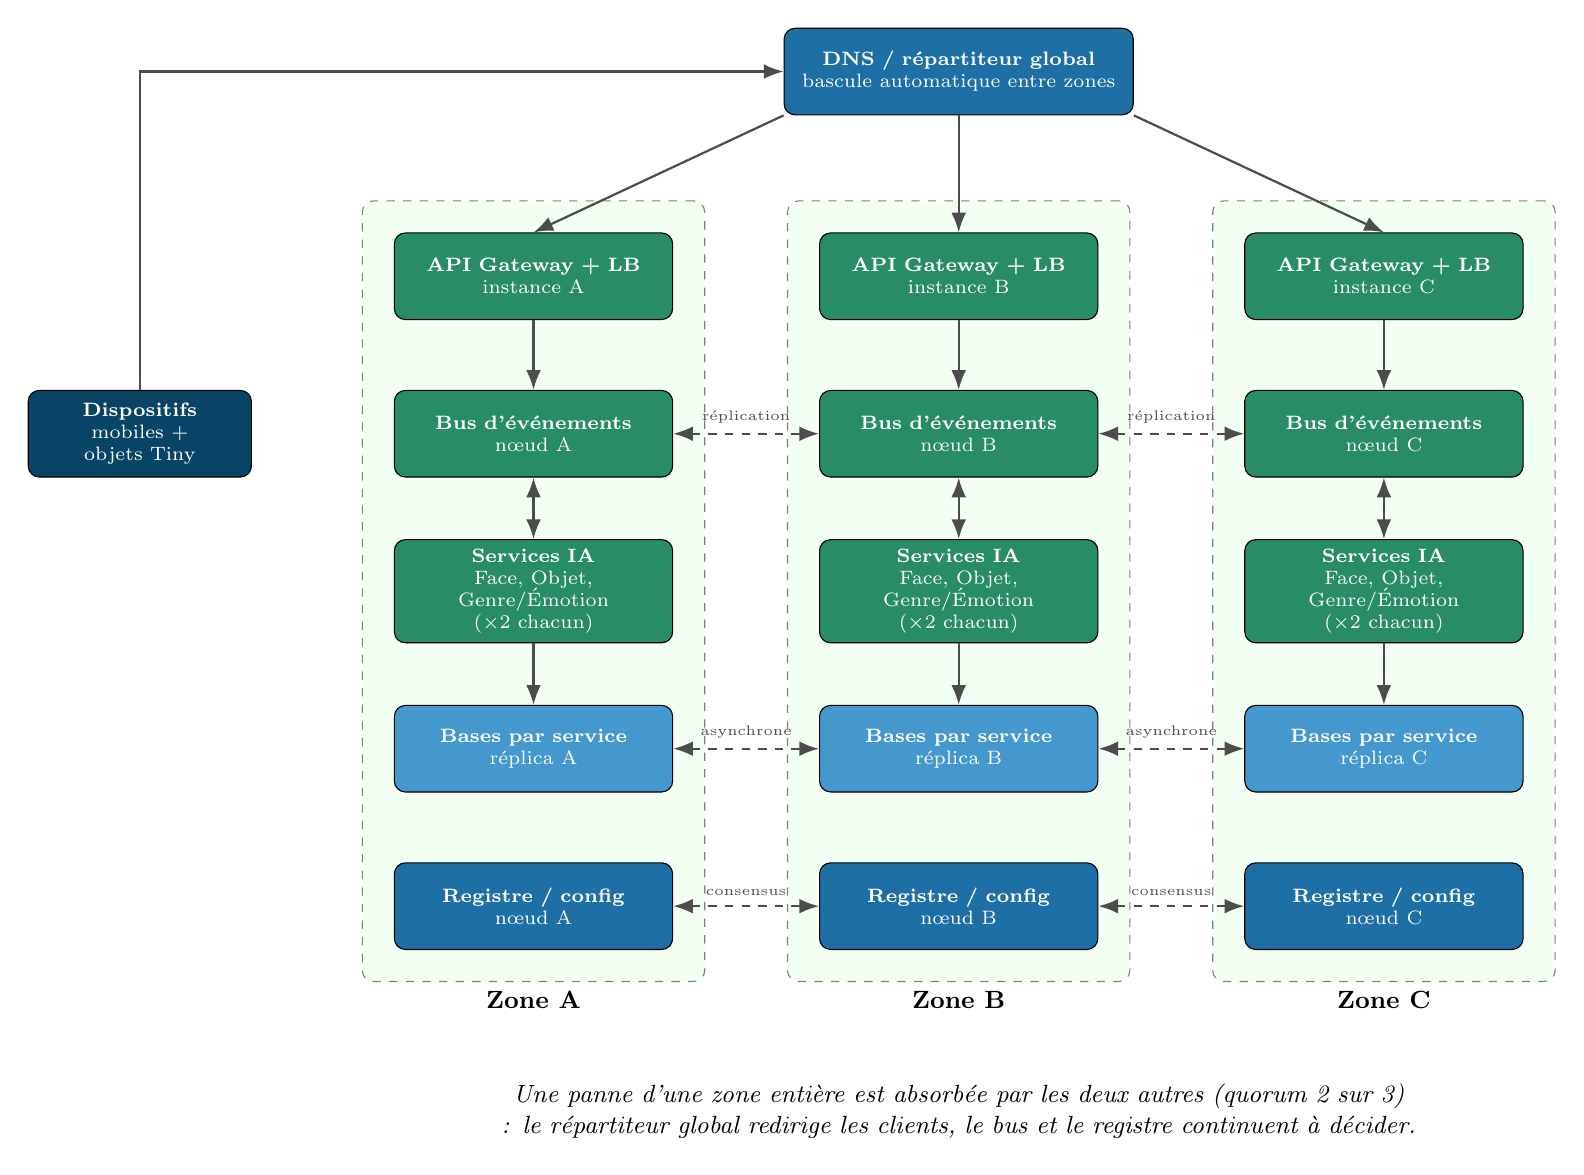
\begin{tikzpicture}[every node/.style={align=center}]
\tikzstyle{nb}=[rectangle, rounded corners, draw=black, text=white, font=\scriptsize, text width=3.3cm, minimum height=1.1cm, align=center]

\node[nb, fill=c4person, text width=2.6cm] (dev) at (0,2.2) {\textbf{Dispositifs}\\ mobiles + objets Tiny};
\node[nb, fill=c4system, text width=4.2cm] (glb) at (10.4,6.8) {\textbf{DNS / répartiteur global}\\ bascule automatique entre zones};

% Zone A
\node[nb, fill=c4new] (gwA) at (5,4.2) {\textbf{API Gateway + LB}\\ instance A};
\node[nb, fill=c4new] (busA) at (5,2.2) {\textbf{Bus d'événements}\\ nœud A};
\node[nb, fill=c4new] (svcA) at (5,0.2) {\textbf{Services IA}\\ Face, Objet, Genre/Émotion\\ ($\times$2 chacun)};
\node[nb, fill=c4system] (regA) at (5,-3.8) {\textbf{Registre / config}\\ nœud A};
\node[nb, fill=c4container] (dbA) at (5,-1.8) {\textbf{Bases par service}\\ réplica A};

% Zone B
\node[nb, fill=c4new] (gwB) at (10.4,4.2) {\textbf{API Gateway + LB}\\ instance B};
\node[nb, fill=c4new] (busB) at (10.4,2.2) {\textbf{Bus d'événements}\\ nœud B};
\node[nb, fill=c4new] (svcB) at (10.4,0.2) {\textbf{Services IA}\\ Face, Objet, Genre/Émotion\\ ($\times$2 chacun)};
\node[nb, fill=c4system] (regB) at (10.4,-3.8) {\textbf{Registre / config}\\ nœud B};
\node[nb, fill=c4container] (dbB) at (10.4,-1.8) {\textbf{Bases par service}\\ réplica B};

% Zone C
\node[nb, fill=c4new] (gwC) at (15.8,4.2) {\textbf{API Gateway + LB}\\ instance C};
\node[nb, fill=c4new] (busC) at (15.8,2.2) {\textbf{Bus d'événements}\\ nœud C};
\node[nb, fill=c4new] (svcC) at (15.8,0.2) {\textbf{Services IA}\\ Face, Objet, Genre/Émotion\\ ($\times$2 chacun)};
\node[nb, fill=c4system] (regC) at (15.8,-3.8) {\textbf{Registre / config}\\ nœud C};
\node[nb, fill=c4container] (dbC) at (15.8,-1.8) {\textbf{Bases par service}\\ réplica C};

% liens verticaux dans chaque zone
\foreach \z in {A,B,C}{
  \draw[arr] (gw\z) -- (bus\z);
  \draw[biarr] (bus\z) -- (svc\z);
  \draw[arr] (svc\z) -- (db\z);
}

% liens entre zones (réplication)
\draw[biarr, dashed] (busA.east) -- node[above, font=\tiny] {réplication} (busB.west);
\draw[biarr, dashed] (busB.east) -- node[above, font=\tiny] {réplication} (busC.west);
\draw[biarr, dashed] (regA.east) -- node[above, font=\tiny] {consensus} (regB.west);
\draw[biarr, dashed] (regB.east) -- node[above, font=\tiny] {consensus} (regC.west);
\draw[biarr, dashed] (dbA.east) -- node[above, font=\tiny] {asynchrone} (dbB.west);
\draw[biarr, dashed] (dbB.east) -- node[above, font=\tiny] {asynchrone} (dbC.west);

% accès
\draw[arr] (dev.north) |- (glb.west);
\draw[arr] (glb.south) -- (gwB.north);
\draw[arr] (glb.south west) -- (gwA.north);
\draw[arr] (glb.south east) -- (gwC.north);

% zones
\begin{scope}[on background layer]
\node[draw=black!50, dashed, rounded corners, fill=green!5, fit=(gwA)(busA)(svcA)(regA)(dbA), inner sep=0.4cm, label={[font=\bfseries\small]below:Zone A}] {};
\node[draw=black!50, dashed, rounded corners, fill=green!5, fit=(gwB)(busB)(svcB)(regB)(dbB), inner sep=0.4cm, label={[font=\bfseries\small]below:Zone B}] {};
\node[draw=black!50, dashed, rounded corners, fill=green!5, fit=(gwC)(busC)(svcC)(regC)(dbC), inner sep=0.4cm, label={[font=\bfseries\small]below:Zone C}] {};
\end{scope}

\node[font=\small\itshape, text width=14cm] at (10.4,-6.4) {Une panne d'une zone entière est absorbée par les deux autres (quorum 2 sur 3) : le répartiteur global redirige les clients, le bus et le registre continuent à décider.};

\end{tikzpicture}
}
\caption{Vue de déploiement de la nouvelle architecture : cloud réparti sur trois zones}
\end{figure}

\subsection{Scénario dynamique : le parcours d'une image}

Le diagramme de séquence ci-dessous illustre une image traitée de bout en bout, y compris l'ordre des échanges et ce qui se passe en cas de lenteur ou de panne.

\begin{figure}[h]
\centering
\resizebox{\textwidth}{!}{%
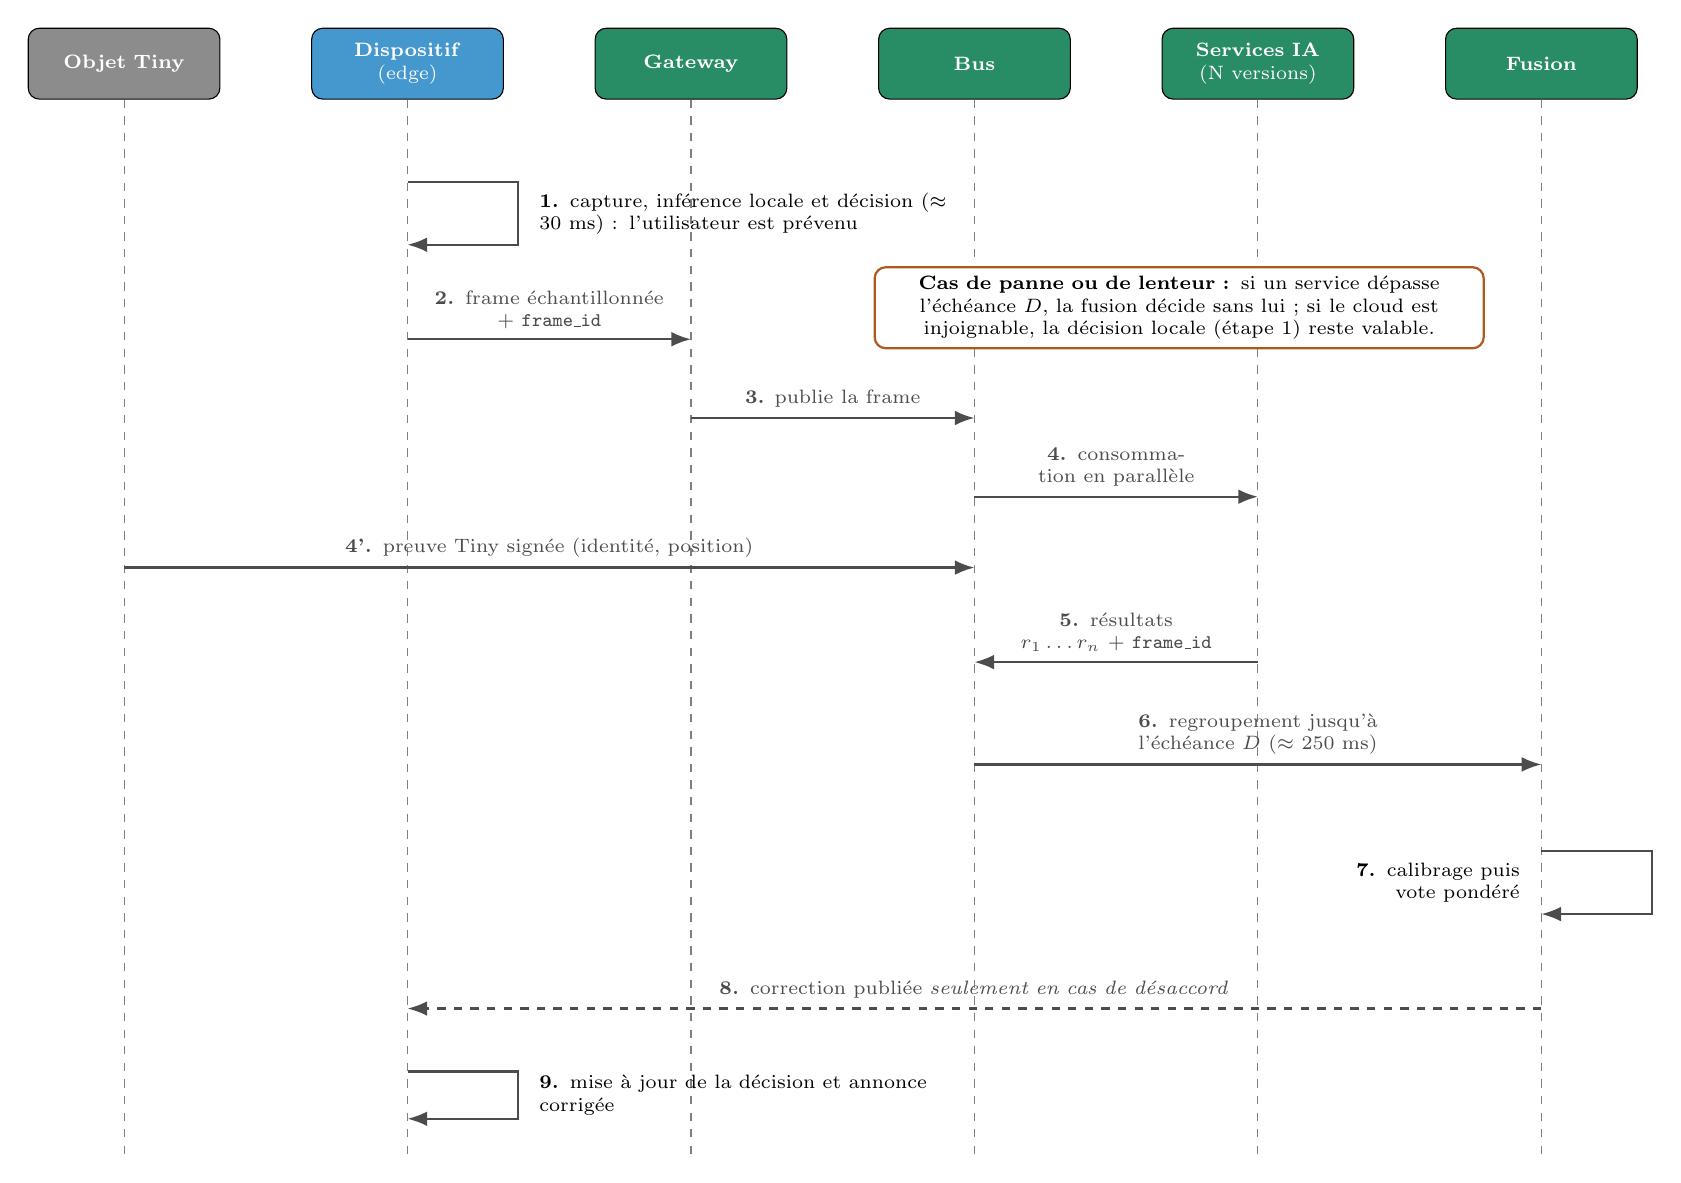
\begin{tikzpicture}[every node/.style={align=center}]
\tikzstyle{pt}=[rectangle, rounded corners, draw=black, text=white, font=\scriptsize, text width=2.2cm, minimum height=0.9cm, align=center]

\node[pt, fill=c4external] (tiny) at (0,0) {\textbf{Objet Tiny}};
\node[pt, fill=c4container] (mob) at (3.6,0) {\textbf{Dispositif}\\ (edge)};
\node[pt, fill=c4new] (gw) at (7.2,0) {\textbf{Gateway}};
\node[pt, fill=c4new] (bus) at (10.8,0) {\textbf{Bus}};
\node[pt, fill=c4new] (svc) at (14.4,0) {\textbf{Services IA}\\ (N versions)};
\node[pt, fill=c4new] (fus) at (18.0,0) {\textbf{Fusion}};

\foreach \n in {tiny,mob,gw,bus,svc,fus}{
  \draw[dashed, gray] (\n.south) -- ++(0,-13.4);
}

% 1 : décision locale
\draw[arr] (3.6,-1.5) -- (5.0,-1.5) -- (5.0,-2.3) -- (3.6,-2.3);
\node[font=\scriptsize, anchor=west, text width=5.2cm, align=left] at (5.15,-1.9) {\textbf{1.} capture, inférence locale et décision ($\approx$ 30 ms) : l'utilisateur est prévenu};

% 2 : envoi asynchrone
\draw[arr] (3.6,-3.5) -- node[above, font=\scriptsize, text width=3.2cm] {\textbf{2.} frame échantillonnée + \texttt{frame\_id}} (7.2,-3.5);
\draw[arr] (7.2,-4.5) -- node[above, font=\scriptsize] {\textbf{3.} publie la frame} (10.8,-4.5);
\draw[arr] (10.8,-5.5) -- node[above, font=\scriptsize, text width=3.2cm] {\textbf{4.} consommation en parallèle} (14.4,-5.5);
\draw[arr] (0,-6.4) -- node[above, font=\scriptsize, text width=6cm] {\textbf{4'.} preuve Tiny signée (identité, position)} (10.8,-6.4);

% 5 : résultats
\draw[arr] (14.4,-7.6) -- node[above, font=\scriptsize, text width=3.2cm] {\textbf{5.} résultats $r_1 \ldots r_n$ + \texttt{frame\_id}} (10.8,-7.6);
\draw[arr] (10.8,-8.9) -- node[above, font=\scriptsize, text width=6cm] {\textbf{6.} regroupement jusqu'à l'échéance $D$ ($\approx$ 250 ms)} (18.0,-8.9);

% 7 : fusion
\draw[arr] (18.0,-10.0) -- (19.4,-10.0) -- (19.4,-10.8) -- (18.0,-10.8);
\node[font=\scriptsize, anchor=east, text width=3.6cm, align=right] at (17.85,-10.4) {\textbf{7.} calibrage puis vote pondéré};

% 8 : correction
\draw[arr, dashed] (18.0,-12.0) -- node[above, font=\scriptsize, text width=7cm] {\textbf{8.} correction publiée \textit{seulement en cas de désaccord}} (3.6,-12.0);

% 9 : mise à jour
\draw[arr] (3.6,-12.8) -- (5.0,-12.8) -- (5.0,-13.4) -- (3.6,-13.4);
\node[font=\scriptsize, anchor=west, text width=5.2cm, align=left] at (5.15,-13.1) {\textbf{9.} mise à jour de la décision et annonce corrigée};

\node[draw=c4warn, thick, rounded corners, font=\scriptsize, fill=white, text width=7.5cm] at (13.4,-3.1) {\textbf{Cas de panne ou de lenteur :} si un service dépasse l'échéance $D$, la fusion décide sans lui ; si le cloud est injoignable, la décision locale (étape 1) reste valable.};

\end{tikzpicture}
}
\caption{Diagramme de séquence : traitement d'une image dans la nouvelle architecture}
\end{figure}

La chronologie à retenir : décision locale en quelques dizaines de millisecondes ; vote cloud en quelques centaines de millisecondes ; correction poussée uniquement si le cloud n'est pas d'accord avec la décision locale.

\subsection{Diagramme C4 -- Niveau 3 : Composants du service de Fusion}

Le service de Fusion remplace le Manager collectif de l'article, c'est le cœur de l'idée « collective ». Ses composants montrent comment une décision est construite à partir de résultats \emph{asynchrones, éventuellement tardifs ou dupliqués}.

\begin{figure}[h]
\centering
\resizebox{\textwidth}{!}{%
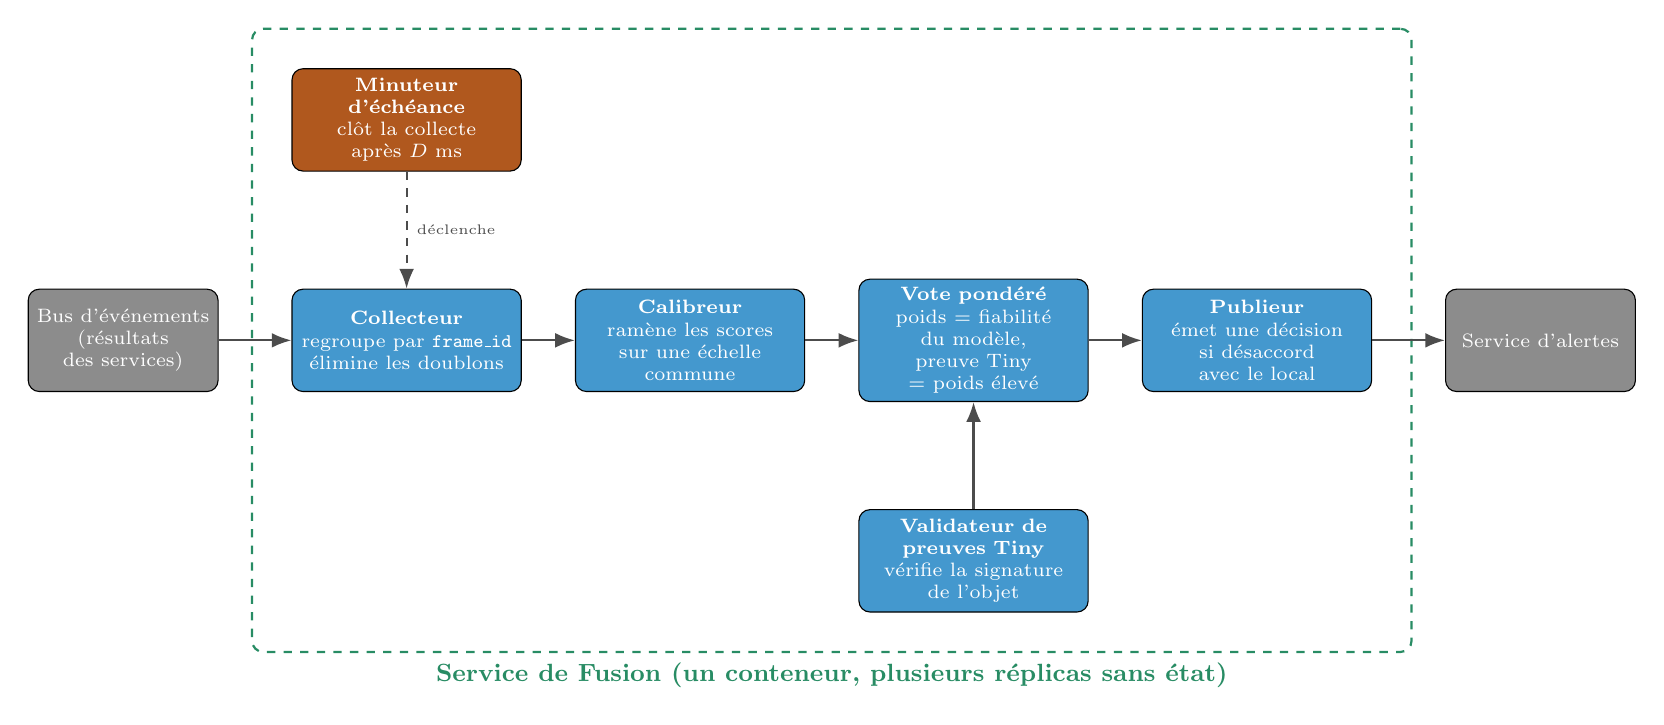
\begin{tikzpicture}[every node/.style={align=center}]

\node[tb, fill=c4external, text width=2.2cm] (in) at (0,0) {Bus d'événements\\ (résultats des services)};
\node[tb, fill=c4container, text width=2.7cm] (col) at (3.6,0) {\textbf{Collecteur}\\ regroupe par \texttt{frame\_id}\\ élimine les doublons};
\node[tb, fill=c4container, text width=2.7cm] (cal) at (7.2,0) {\textbf{Calibreur}\\ ramène les scores\\ sur une échelle commune};
\node[tb, fill=c4container, text width=2.7cm] (vote) at (10.8,0) {\textbf{Vote pondéré}\\ poids = fiabilité du modèle,\\ preuve Tiny = poids élevé};
\node[tb, fill=c4container, text width=2.7cm] (pub) at (14.4,0) {\textbf{Publieur}\\ émet une décision\\ si désaccord avec le local};
\node[tb, fill=c4external, text width=2.2cm] (out) at (18.0,0) {Service d'alertes};

\node[tb, fill=c4warn, text width=2.7cm] (timer) at (3.6,2.8) {\textbf{Minuteur d'échéance}\\ clôt la collecte\\ après $D$ ms};
\node[tb, fill=c4container, text width=2.7cm] (val) at (10.8,-2.8) {\textbf{Validateur de preuves Tiny}\\ vérifie la signature\\ de l'objet};

\draw[arr] (in) -- (col);
\draw[arr] (col) -- (cal);
\draw[arr] (cal) -- (vote);
\draw[arr] (vote) -- (pub);
\draw[arr] (pub) -- (out);
\draw[arr, dashed] (timer) -- node[right, font=\tiny] {déclenche} (col);
\draw[arr] (val) -- (vote);

\begin{scope}[on background layer]
\node[draw=c4new, thick, dashed, rounded corners, fit=(col)(cal)(vote)(pub)(timer)(val), inner sep=0.5cm, label={[c4new, font=\bfseries\small]below:Service de Fusion (un conteneur, plusieurs réplicas sans état)}] {};
\end{scope}

\end{tikzpicture}
}
\caption{Diagramme C4 -- Niveau Composants du service de Fusion}
\end{figure}

\subsection{Mécanismes de répartition}

\subsubsection{Propriétés des systèmes répartis et mécanismes retenus}

\begin{table}[h]
\centering
\begin{tabular}{|p{3.0cm}|p{11.6cm}|}
\hline
\textbf{Propriété} & \textbf{Mécanisme dans la nouvelle architecture} \\
\hline
Hétérogénéité & Protocole adapté à chaque tier : MQTT pour les objets Tiny, gRPC ou MQTT entre dispositif et cloud, messages sur le bus entre services \\
\hline
Concurrence & Consommation parallèle d'un même événement par N versions de modèles ; services sans état, donc réplicables librement \\
\hline
Horloge globale & Chaque image reçoit un \texttt{frame\_id} unique et un horodatage ; les résultats sont fusionnés par \texttt{frame\_id} et non par ordre d'arrivée ; horloges synchronisées par NTP \\
\hline
Pannes partielles & Échéance $D$ sur la collecte, \textit{timeouts}, reprises avec \textit{backoff}, \textit{circuit breaker}, réplication des services, du bus et du registre sur trois zones \\
\hline
Transparence & Le registre de services masque la localisation ; le répartiteur global masque la zone ; le client ignore combien de réplicas existent \\
\hline
Passage à l'échelle & Services sans état, ajout de réplicas selon la charge, topics du bus partitionnés par client (l'ordre est conservé pour un client donné) \\
\hline
Sécurité & Authentification au Gateway, mTLS entre services, certificat par objet Tiny, envoi d'\textit{embeddings} plutôt que d'images \\
\hline
Ouverture & Ajouter une version de modèle = déployer un nouveau conteneur abonné au même sujet, sans modifier le reste \\
\hline
\end{tabular}
\caption{Réponse de la nouvelle architecture aux propriétés des systèmes répartis}
\end{table}

\subsubsection{Choix de cohérence (théorème CAP)}

Lors d'une partition du réseau, un système réparti doit choisir entre \emph{cohérence} (tous voient la même donnée) et \emph{disponibilité} (il répond toujours). Le choix est fait \emph{donnée par donnée}.

\begin{table}[h]
\centering
\begin{tabular}{|p{4.2cm}|p{2.6cm}|p{7.8cm}|}
\hline
\textbf{Donnée} & \textbf{Choix} & \textbf{Justification} \\
\hline
Résultats d'inférence, alertes & Disponibilité, cohérence à terme (AP) & Une correction légèrement en retard est acceptable ; l'absence de réponse ne l'est pas, et la décision locale existe déjà \\
\hline
Registre de services, configuration, version active d'un modèle & Cohérence forte (CP), par consensus et quorum & Un routage ou une version erronés sont pires qu'une courte indisponibilité \\
\hline
Dataset de visages, embeddings & Cohérence à terme, données versionnées & Les mises à jour sont rares et peuvent se propager de façon asynchrone \\
\hline
\end{tabular}
\caption{Cohérence choisie selon la nature de la donnée}
\end{table}

\subsubsection{Modes de fonctionnement}

\begin{table}[h]
\centering
\begin{tabular}{|p{3.3cm}|p{11.3cm}|}
\hline
\textbf{Situation} & \textbf{Comportement du système} \\
\hline
Nominal & Décision locale immédiate, puis correction cloud avant l'échéance $D$ \\
\hline
Cloud lent & L'échéance $D$ est dépassée : la fusion décide sans les retardataires ; une correction devenue périmée (image trop ancienne) est ignorée \\
\hline
Panne d'un service ou d'un réplica & Le \textit{circuit breaker} s'ouvre, le vote se fait avec les versions restantes, les poids sont renormalisés ; le réplica est relancé automatiquement \\
\hline
Panne d'une zone & Le répartiteur global redirige vers les deux autres zones ; le quorum 2 sur 3 est conservé \\
\hline
Hors ligne (partition) & Décision locale seule ; événements conservés dans la file locale ; resynchronisation au retour du réseau, sans doublons grâce à l'idempotence \\
\hline
\end{tabular}
\caption{Modes de fonctionnement nominal et dégradés}
\end{table}

\subsection{Correspondance entre l'architecture de l'article et la nouvelle}

\begin{table}[h]
\centering
\begin{tabular}{|p{5.6cm}|p{9.0cm}|}
\hline
\textbf{Élément de l'article} & \textbf{Dans la nouvelle architecture} \\
\hline
Client \textit{lite} (\textit{DNN//c}) & Tier edge : modèles quantifiés, manager local, décision immédiate \\
\hline
Serveur multi-versions (\textit{DNN//s}) & Services d'inférence conteneurisés, répliqués sur trois zones \\
\hline
Gateway REST unique & Load Balancer + API Gateway en plusieurs instances \\
\hline
Appels REST synchrones & Bus d'événements (publish/subscribe) et gRPC en flux \\
\hline
\texttt{MSParallelCollectiveManager} & Service de Fusion : échéance, calibrage, vote pondéré \\
\hline
\texttt{ManagerServer} et envoi d'alerte & Service d'alertes : correction poussée seulement si désaccord \\
\hline
\texttt{MSTinyParallelCollective} (Arduino) & Objets Tiny publiant des preuves signées sur MQTT \\
\hline
\texttt{MSFaceDynamicTraining} + redémarrage & Registre de modèles et MLOps : déploiement progressif sans coupure \\
\hline
« Un service par processeur » & Autoscaling de réplicas sans état \\
\hline
Dataset partagé & Une base par service, réplication, cohérence à terme \\
\hline
\end{tabular}
\caption{Correspondance entre l'ancien et le nouveau}
\end{table}

\subsection{Choix technologiques indicatifs}

Ces technologies illustrent les rôles ; elles sont remplaçables par des équivalents.

\begin{table}[h]
\centering
\begin{tabular}{|p{4.2cm}|p{10.4cm}|}
\hline
\textbf{Rôle} & \textbf{Exemple} \\
\hline
Liaison objets Tiny & MQTT sur TLS \\
\hline
Inférence sur le dispositif & Modèles quantifiés au format TensorFlow Lite ou ONNX \\
\hline
Bus d'événements & Kafka, ou RabbitMQ / Mosquitto pour un prototype \\
\hline
Services & Conteneurs Docker ; orchestration par Kubernetes (Docker Compose pour un prototype) \\
\hline
Registre de services et configuration & Consul ou etcd (consensus à quorum) \\
\hline
Observabilité & Prometheus, Grafana, OpenTelemetry \\
\hline
Registre de modèles / MLOps & MLflow \\
\hline
\end{tabular}
\caption{Technologies indicatives}
\end{table}

\subsection{Compromis et risques}

Aucune architecture n'est parfaite ; il faut le dire pour montrer le recul.

\begin{itemize}
    \item \textbf{Complexité d'exploitation} : bus répliqué, orchestration, consensus exigent des compétences d'exploitation. Pour un prototype, on peut se limiter à deux réplicas, Docker Compose et un seul broker MQTT, en gardant la même logique.
    \item \textbf{Coût} : trois zones et des GPU dans le cloud coûtent plus qu'un seul serveur.
    \item \textbf{Cohérence perçue} : l'utilisateur peut entendre une annonce puis sa correction. On limite ce risque en n'annonçant localement que les décisions à forte confiance.
    \item \textbf{Latence ajoutée par le bus} : acceptable car le chemin critique (décision locale) ne passe jamais par le bus.
    \item \textbf{Hypothèse Tiny} : la preuve des objets suppose qu'ils soient connectés, ce qui n'est pas toujours réaliste ; le système reste fonctionnel sans elle, avec une précision moindre.
\end{itemize}

% ======================================================================
\section{Partie 3 -- Idées de validation de la nouvelle architecture}
% ======================================================================

Valider, c'est démontrer que l'architecture répond mieux aux exigences que l'existant, et en particulier qu'elle remplit désormais les critères d'un système réparti. Pistes proposées :

\begin{enumerate}
    \item \textbf{Vérification des 5 critères microservices et des 8 propriétés réparties.} Reprendre les deux tableaux de la partie 1 et vérifier que chaque case passe de « Non » à « Oui » (par exemple, redéployer le seul service Face sans interrompre les autres). 

    \item \textbf{Tests de charge.} Simuler un nombre croissant de clients simultanés (JMeter, Locust) et mesurer temps de réponse et débit avant/après. \textit{Succès :} temps de réponse stable quand les clients augmentent.

    \item \textbf{Tests de résilience (\textit{chaos engineering}).} Arrêter volontairement un réplica, puis un service entier, et vérifier que la décision collective continue. \textit{Succès :} aucune interruption perçue, contrairement à l'existant où un maillon cassé arrête la chaîne.

    \item \textbf{Bascule de zone.} Couper une zone entière et mesurer le temps de bascule du répartiteur global. \textit{Succès :} service rétabli en quelques secondes, quorum conservé.

    \item \textbf{Partition réseau et mode hors ligne.} Couper le réseau entre le dispositif et le cloud, vérifier que la décision locale continue, puis que la resynchronisation s'effectue au retour. \textit{Succès :} aucune perte, aucune décision dupliquée.

    \item \textbf{Injection de latence et d'échéance.} Ralentir artificiellement un service et vérifier que la fusion décide à l'échéance $D$ sans lui. \textit{Succès :} délai de décision borné.

    \item \textbf{Doublons et idempotence.} Rejouer les mêmes messages et vérifier qu'ils ne sont traités qu'une fois. \textit{Succès :} zéro double traitement.

    \item \textbf{Reproduction du protocole expérimental de l'article.} Rejouer Multi-PIE, Bosphorus et YouTube-BoundingBoxes et comparer les matrices de confusion. \textit{Succès :} précision identique ou meilleure, ce qui prouve que la répartition n'a pas dégradé le résultat algorithmique.

    \item \textbf{Tests de sécurité.} Faire publier un objet Tiny non authentifié ou avec une signature falsifiée, et vérifier qu'il est rejeté ; vérifier le chiffrement des échanges.

    \item \textbf{Revue d'architecture (ATAM simplifiée) et prototype.} Confronter l'architecture à des scénarios (« une zone tombe », « 1000 utilisateurs arrivent ») avec enseignant et camarades, puis déployer une maquette à quelques conteneurs (Gateway, deux services, un broker) pour démontrer la faisabilité.
\end{enumerate}

\subsection{Indicateurs cibles}

Les valeurs ci-dessous sont des \textbf{hypothèses de travail à calibrer par la mesure}, elles ne proviennent pas de l'article.

\begin{table}[h]
\centering
\begin{tabular}{|p{6.6cm}|p{4.0cm}|p{3.8cm}|}
\hline
\textbf{Indicateur} & \textbf{Cible proposée} & \textbf{Test associé} \\
\hline
Latence de la décision locale (95\textsuperscript{e} percentile, hors réseau) & $<$ 50 ms & Mesure sur dispositif \\
\hline
Délai de correction cloud (95\textsuperscript{e} percentile, échéance incluse) & $<$ 500 ms & Tests de charge \\
\hline
Disponibilité de la décision locale en cas de coupure réseau & 100\% & Partition réseau \\
\hline
Perte de messages lors de la panne d'un nœud du bus & 0 & Chaos engineering \\
\hline
Temps de bascule après perte d'une zone & $<$ 30 s & Bascule de zone \\
\hline
Messages traités deux fois & 0 & Doublons et idempotence \\
\hline
Précision (matrices de confusion) & $\geq$ architecture initiale & Reproduction du protocole \\
\hline
\end{tabular}
\caption{Indicateurs cibles pour valider l'architecture}
\end{table}

% ======================================================================
\section{Conclusion}
% ======================================================================

L'analyse de l'article montre une architecture à lire à deux niveaux. Globalement, il s'agit d'une \textbf{architecture client-serveur à client lourd, étendue à trois tiers} par des objets connectés. Au niveau de l'implémentation, malgré le vocabulaire « micro-services », le prototype est un \textbf{monolithe modulaire multi-processus} exécuté sur une seule machine, qui ne remplit aucun des cinq critères d'un microservice. Vu comme système réparti, il est distribué géographiquement sans avoir été conçu pour la répartition : pannes partielles, horloge globale, cohérence, transparence et sécurité ne sont pas traitées.

La nouvelle architecture migre la solution vers un \textbf{système réparti hybride}. Elle \textbf{conserve ce qui fonctionne} -- la relation client lourd / serveur correcteur, les objets Tiny, l'idée de collectif -- et la reconstruit sur quatre piliers : un \textbf{continuum Edge--Cloud} (décision locale d'abord), des \textbf{microservices réellement indépendants}, un \textbf{bus d'événements} qui découple les échanges, et une \textbf{réplication sur trois zones} avec des choix de cohérence explicites. Le service de Fusion, calibré et borné par une échéance, remplace le Manager naïf. Les pistes de validation, centrées sur les pannes, les partitions et les doublons, permettent de démontrer par l'expérience que cette répartition est maîtrisée, sans sacrifier la précision de la solution d'origine.

\end{document}
